%%%%%%%%%%%%%%%%%%%%%%%%%%%%%%%%%%%%%%%%%%%%%%%%%%%%%%%%%%%%%%%%%%%%%%%%%%%%%%
%
% Main content starts here
%
%%%%%%%%%%%%%%%%%%%%%%%%%%%%%%%%%%%%%%%%%%%%%%%%%%%%%%%%%%%%%%%%%%%%%%%%%%%%%%

\pagenumbering{arabic}
\chapter{Introduction}
\label{sec:introduction}


\section{Background and Motivation}

Programming is an essential part of computer science and it is defined as one of the most difficult process to learn. \cite{andrzejewska2020development} It is considered as a cognitive activity that use various kinds of mental models, in order to understand the semantics and syntax of the programming language \cite{andrzejewska2020development}.
Furthermore, correctly understandable abstract concepts are also a key part of the programming process \cite{lahtinen2005study}.

There are various studies that investigate expert programmers. These studies define expert as people who use effective strategies \cite{robins2003learning}.   Experts tend to spent more time planning and testing code. In contrast, novices do not have the same skills as experts and are defined as beginner in programming \cite{robins2003learning} Novices tend to spend less time planning and testing code. Moreover, beginners have less knowledge about the sequential nature of execution of programs and have difficulties understanding some code language constructs \cite{robins2003learning}.


Recently, many students have an interest in pursuing computer science. Therefore, introductory programming courses (CS1) have gained popularity in the education. \cite{robins2003learning}. In general, programming courses are considered difficult with highest dropout rates \cite{robins2003learning} It is considered that psychological and social factors, which are related to the perception of programming, are among the main difficulties of the programming process \cite{andrzejewska2020development}. Introductory programming courses present only the basic concepts of programming, and their goal is to teach how to write good code. However, code comprehension and quality topic are discussed later in the education process \cite{ inproceedings}.

Code comprehension is defined as a key part of programming concepts and as one of the most time-consuming tasks \cite{javier2021understanding}.
Recent research discusses how code formatting affects code comprehension and whether correct code structure makes it more understandable \cite{andrzejewska2020development}. It is considered that indentation affects program comprehension. Indentation decreases the time spent on source code, making the code structure easier to perceive \cite{bauer2017indentations}. Furthermore, code comments are also consider to have an impact on code comprehension. Comments describe the functionality of the code, making the code more understandable \cite{bakhuizen2019comments}.
 
Usually, beginners are poor at tracking code, and their code comprehension is affected by how information is presented \cite{robins2003learning}. Some research aims to discover how poorly indented or poorly commented code has an influence on cognitive load and code comprehension.  However, eye-tacking studies on the effects of commenting and indentations on code comprehension among beginners have been rare so far and still remain a gap in computer science education.

  
This thesis presents an eye-tracking study, investigating the effects of indentation and commenting formats on novices’ perception of code and cognitive load. Eye-tacking technology helps visualize the eye movements of beginners and detect their cognitive load. 


\section{Research question}

The central research question in the thesis is: \textbf{RQ1.1:} How do commenting formats and indentation level affect code comprehension among CS1 students? To answer this question, the following sub-questions should be considered:

\begin{itemize}
    \item \textbf{RQ1.2:} Do well-indented code snippets lead to better comprehension?
    \item \textbf{RQ1.3:} Does random indentation and redundant comments increase cognitive load?
    \item \textbf{RQ1.4:} How does the time spent reading code vary between different commenting formats?
    \item \textbf{RQ1.5:} How does the time spent reading code vary between different levels of indentation?
\end{itemize}

These questions help to provide insights into the role of code indentation and commenting in code comprehension. 
To answer them, this thesis presents a study that focuses on the effects of code indentation and commenting on code comprehension among CS1 students.
The study consists of two formats: an offline study using eye-tracking technology and an online study without eye-tracking. Both formats use the same questionnaire. The questionnaire consists of seven code snippets and several questions related to each snippet. The questionnaire gathers information about the participants, such as their understanding of the snippets, while the eye-tracking technology gathers data, such as participants’ gaze patterns and cognitive load during code reading.  

\section{Thesis organization and contributions}

The thesis is organized as follows:
\begin{itemize}

\item[] \emph{Chapter 2:} 
\\This chapter gives an overview of the theoretical background of code readability and code comprehension. Additionally, the Cognitive Load Theory and the Theory of Program Comprehension are presented to address human understanding. The Cognitive Load Theory discusses how the visual presentation of information  affect mental processes and Theory of Program Comprehension discuss how programmers interpret code. 
Furthermore, the chapter discusses the eye-tracking approach and eye-tracking studies.  


\item[] \emph{Chapter 3:}
\\This chapter presents the design of the study. It describes the technical setup, code snippets selection, and how data was collected. Additionally, details on study conditions and ethical considerations are included.


\item[] \emph{Chapter 4:} 
\\ This chapter presents the findings of the study. The results are based on the data collected from the eye-tracking device and questionnaire. The eye-tracking data is presented using heatmaps and gaze plots.


\item[] \emph{Chapter 5:} 
\\In this chapter, the results from the study are interpreted. In addition, it is discussed how indentation and comments influenced the code comprehension of participants. Additionally, the limitations and possible improvements are included.

\item[] \emph{Chapter 6:} 
\\The final chapter summarizes the main findings of the thesis. Furthermore, it also presents directions for future research.

\end{itemize}


In this thesis, the following contributions are made:
\begin{enumerate}

\item The thesis presents a replicable study, which combines eye-tracking technology and questionnaire. Eye-tracking data gave information about the gaze patterns and cognitive load of the participants. The questionnaire presented participants’ opinion about code comprehension.

\item  The conducted study investigates the effects of different levels of indentation and commenting formats on code comprehension among CS1 students. The results of the study are discussed and present overview of which levels of indentation and commenting formats improve code comprehension.

\item The conducted study can be used for developing better coding guidelines for CS1 students.

\end{enumerate}

\chapter{Literature Review}
In this chapter, we present the theoretical background of the basic concepts of the thesis. Moreover, we define and explain different ....


\section{Quality}
The quality is defined by several International organisations.

German Industry Standard DIN 55350 Part 11 defines, that the quality “ … comprises all characteristics and significant features of a product or an activity which relate to the satisfying of given requirements” \cite{fitzpatrick1996software}.

Another definition of quality is presented in ANSI Standard (ANSI/ASQC A3/1978), describing that the "Quality is the totality of features and characteristics of a product or a service that bears on its ability to satisfy the given needs"  \cite{fitzpatrick1996software}.

ANOTHER DEFITION comes later....

\section{Quality models}

\subsection{Quality model ISO 9126-1}
text text
e

de
de
de


\begin{longtable}{p{0.3\textwidth} | p{0.65\textwidth}}
    \caption{Sub-characteristics of the ISO 9126-1 quality model.} \label{tab:table1} \\
    \textbf{Quality Characteristics} & \textbf{Sub-characteristics} \\
    \hline
    \endfirsthead

    \multicolumn{2}{c}%
    {{\bfseries \tablename\ \thetable{} -- continued from previous page}} \\
    \textbf{Quality Characteristics} & \textbf{Sub-characteristics} \\
    \hline
    \endhead

    \hline \multicolumn{2}{r}{{Continued on next page}} \\
    \endfoot

    \hline
    \endlastfoot
    \\
    Functionality & 
    Suitability \newline
    Accuracy \newline
    Interoperability \newline
    Security \newline
    Compliance \\
    \\
    \hline
    \\
    Reliability & 
    Maturity \newline
    Fault tolerance \newline
    Recoverability \newline
    Compliance \\
    \\
    \hline
    \\
    Usability & 
    Understandability \newline
    Learnability \newline
    Operability \newline
    Compliance \\
    \\
    \hline
    \\
    Efficiency & 
    Time behavior \newline
    Resource behavior \newline
    Compliance \\
    \\
    \hline
    \\
    Maintainability & 
    Analyzability \newline
    Changeability \newline
    Stability \newline
    Testability \newline
    Compliance \\
    \\
    \hline
    \\
    Portability & 
    Adaptability \newline
    Installability \newline
    Co-existence \newline
    Replaceability \newline
    Compliance \\
    \\
    
\end{longtable}


\subsection{Quality model ISO 25010 }


textextex
\begin{longtable}{p{0.3\textwidth} | p{0.65\textwidth}}
    \caption{Sub-characteristics of the Quality model - ISO/IEC 25010} \label{tab:table1} \\
    \textbf{Quality Characteristics} & \textbf{Sub-characteristics} \\
    \hline
    \endfirsthead

    \multicolumn{2}{c}%
    {{\bfseries \tablename\ \thetable{} -- continued from previous page}} \\
    \textbf{Quality Characteristics} & \textbf{Sub-characteristics} \\
    \hline
    \endhead

    \hline \multicolumn{2}{r}{{Continued on next page}} \\
    \endfoot

    \hline
    \endlastfoot
    \\
    Functional Suitability & 
    Functional completeness \newline
    Functional correctness \newline
    Functional appropriateness \\
    \\
    
    \hline
    \\
    Reliability &
    Maturity \newline
    Availability \newline
    Fault tolerance \newline
    Recoverability \\
    \\
    \hline
    \\
    Performance Efficiency &
    Time behaviour \newline
    Resource utilization \newline
    Capacity \\
    \\
    \hline
    \\
    Compatibility &
    Co-existence \newline
    Interoperability \\
    \\
    \hline
    \\
    Usability &
    Appropriateness recognizability \newline
    Learnability \newline
    Operability \newline
    User error protection \newline
    User interface aesthetics \newline
    Accessibility \\
    \\
    \hline
    \\
    Security &
    Confidentiality \newline
    Integrity \newline
    Non-repudiation \newline
    Accountability \newline
    Authenticity \\
    \\
    \hline
    \\
    Maintainability &
    Modularity \newline
    Reusability \newline
    Analysability \newline
    Modifiability \newline
    Testability \\
    \\
    \hline
    \\
    Portability &
    Adaptability \newline
    Installability \newline
    Replaceability \\
    \\
\end{longtable}

\section{Code readability}
\section{Code comprehension)}
\section{Indentation}

Indentation is an approach used to organize source code. At the beginning of a code line, there is some space \cite{morzeck2023indentation}.
This method is applied to define code fragments such as loops and conditions.  It can be observed that most of the source code examples in programming education are indented \cite{morzeck2023indentation}. In Java, for instance, it is often required to add a new line after an opening brace, and the lines inside are indented until the closing brace \cite{hanenberg2024indentation}.


The level of indentation can vary in different programming languages and can be set as a personal preference \cite{bauer2017indentations}. Considering the programming language Java, there are many style guides suggestions for which indentation to use. The most commonly used suggestion is an indentation of four spaces. This level of indentation is proposed by style guides such as Oracle and Google \cite{bauer2017indentations}.
Several IDEs, such as Visual Studio and IntelliJ, often use formatting tools that automatically apply indentation to the source code \cite{morzeck2023indentation}.


\begin{figure} [H]
  \centering
  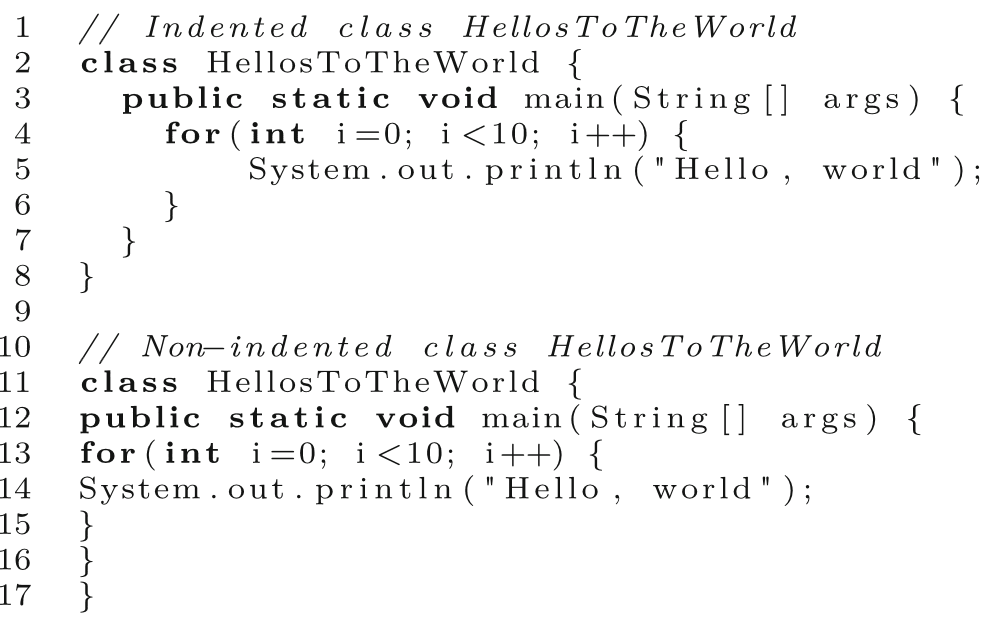
\includegraphics [scale=0.7]
  {figures/indentation_ex.png}
  \caption{Non–indented and indented Java code snippet \cite{hanenberg2024indentation}.}
  \label{fig:AnhangsChor}
\end{figure}

Figure … presents Java code snippet, which gives an output the words “Hello, world”  \cite{hanenberg2024indentation}.
In the first code snippet, which is indented, some space is added before the main method and the loop.  In the second code snippet, which is not indented, no space is added. The additional space visualizes that particular code lines belong to another fragment. In the non-indented code snippet, it is difficult to detect the code structure. 
 





\section{Commenting}


\begin{figure}[H]
\centering
\begin{tikzpicture}[
  base/.style={draw, rounded corners, minimum width=4cm, minimum height=1cm, align=center},
  line/.style={draw, -latex},
  node distance=0.6cm
]

% Subcategories (stacked vertically)
\node[base] (copyright) {Copyright Comments};
\node[base, below=of copyright] (header) {Header Comments};
\node[base, below=of header] (member) {Member Comments};
\node[base, below=of member] (inline) {Inline Comments};
\node[base, below=of inline] (section) {Section Comments};
\node[base, below=of section] (code) {Code Comments};
\node[base, below=of code] (task) {Task Comments};

% Calculate center node (manually placed to center vertically)
\node[base, left=4cm of inline] (main) {Comment Classification};

% Connecting lines
\foreach \node in {copyright, header, member, inline, section, code, task} {
  \draw[line] (main.east) -- (\node.west);
}

\end{tikzpicture}
\caption{Classification of Code Comments}
\label{fig:comment_classification}
\end{figure}




\section{Cognitive Load Theory (CLT)}
- Relevance to Code Comprehension

\section{Theory of Program Comprehension}
- Top-Down Model: Experienced programmers use existing knowledge to understand the structure and intent of code quickly.

- Bottom-Up Model: Beginners read line-by-line, building their understanding incrementally.

- Integrated Model: A mix of both, depending on experience level and task complexity


\begin{figure} [H]
  \centering
  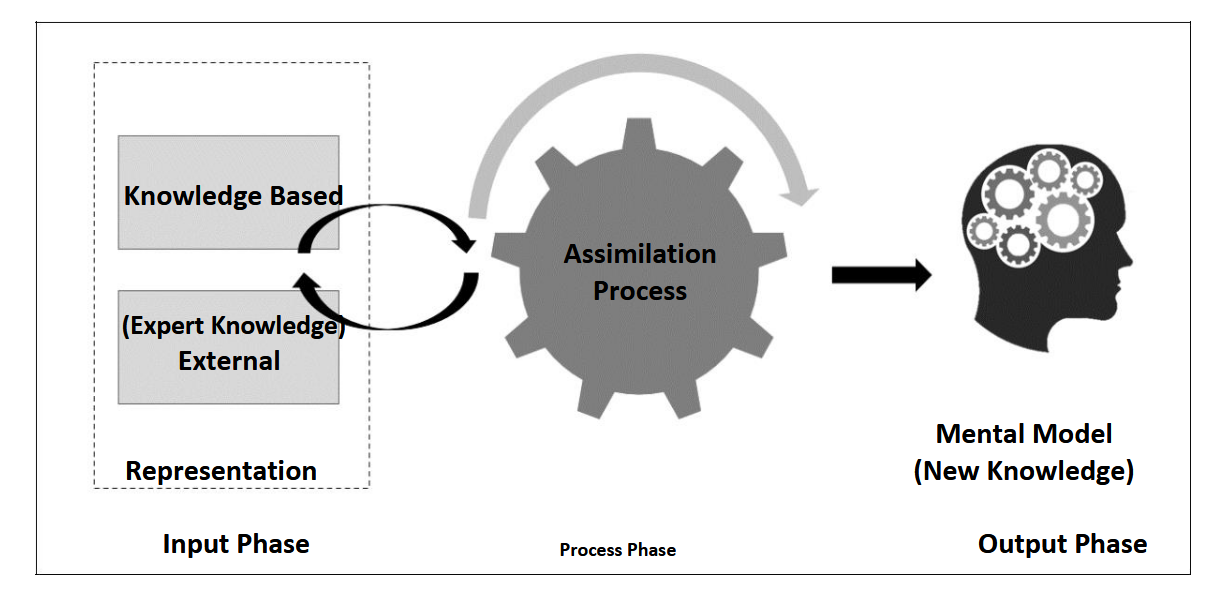
\includegraphics[width=\textwidth]{figures/program_Comprehension_Process.png}
  \caption{The Program Comprehension Process}
  \label{fig:AnhangsChor}
\end{figure}

\section{Eye Tracking}

•	Definition 


•	Background


•	Metrics


•	Why it’s relevant: Eye-tracking studies assume that where a person looks is what they are thinking about.


•	Key ideas:


o	Fixations (longer gaze duration) suggest higher cognitive processing effort.


o	Saccades (quick eye movements) indicate searching behavior (e.g., students scanning comments before reading the code).


o	Areas of Interest (AOI) refer to parts of the stimulus on which eye-tracking metrics are recorded. Examples could be chunks in the code editor, the requirements area of the IDE, or the console output. The AOI is usually defined by the researcher.


•	How to apply it:


o	Compare eye-tracking heatmaps to see if students focus more on comments before reading the code.


o	Measure how indentation influences reading patterns—does better indentation make scanning for logic structures easier?


\section{Studies using Eye Tracking}

Several studies analyze programming comprehension, using eye-tracking technology. This chapter reviews key studies, categorizing them based on their focus areas and summarizing their findings.

\subsubsection{Eye-Tracking Methodologies in Software Engineering}
The paper \citet{obaidellah2018survey} investigates the use of eye-tracking technology in computer programming research. A total of 63 relevant studies published between 1990 and June 2017 are analysed \citet{obaidellah2018survey}. The results indicate that eye-tracking technology has been applied to understand programmers' gaze pattern and cognitive processes. The studies reviewed in this paper focus on five main research fields: program comprehension and code understanding, non-code comprehension studies, debugging, requirements traceability, and collaborative programming \citet{obaidellah2018survey}.  The most frequently studied programming language is Java.  
For eye-tracking system, Tobii is the most commonly used.  Fixation duration and saccades are identified as primary metrics for analysing gaze patterns, and heatmaps are created for visual representation of the results.


\subsubsection{Variable Naming Conventions and Code Readability}

The study \citet{sharif2010eye}investigates whether different variable naming conventions (camel-case and underscore) impact code comprehension and readability.
The task of the participants was to recognize different variable names, while their eye movements were tracked and analysed from the researches. 
The findings indicate no significant difference in accuracy between the camel-case and underscore naming conventions \citet{sharif2010eye}. However, underscore identifiers were recognized 20\% faster compared to camel-case identifiers \citet{sharif2010eye}. Moreover, the data from the eye-tracking technology showed that camel-case identifiers led to longer gaze durations, more fixations, and a   higher cognitive load. Furthermore, novice programmers benefited more from the underscore variable naming conventions.   
Overall, the results indicate that underscore variable naming conventions are easier to process visually and potentially improve code readability.   


The eye-tracking study \citet{broberg2019using}investigates how different variable naming conventions impact on code readability.  
The test subjects analyzed code snippets containing variables in Single Word (SW), Single Letter (SL), Camel Case (MWCC), and Snake Case (MWSC) \citet{broberg2019using}. While explaining the code snippets, their eye movements were tracked. Researchers measured the time participants spent analysing the code and then created heatmaps to visualize their gaze patterns. Furthermore, participants provided feedback on which naming conventions they prefer. The results present no significant differences in readability using different variable naming conventions \citet{broberg2019using}. However, multi-word conventions like Snake Case and Camel Case were easier to read than Single Letter variable naming conventions \citet{broberg2019using}. The heatmaps presented that test subjects spent more time processing single-letter variables, leading to higher cognitive effort. Moreover, most participants personally found Snake Case and Camel Case easier to understand \citet{broberg2019using}. 
This study presents the role of meaningful variable naming conventions in code and how they improve code readability.   

\subsubsection{Code Transformations and Their Impact on Comprehension}
The eye-tracking study \citet{silva2023evaluating} investigates how different code transformations affect novice programmers’ code comprehension \citet{silva2023evaluating}. It focuses on Atoms of Confusion, Refactorings, and ifdef Annotations.

The findings show that confusing code snippets lead to difficulties in code comprehension and in increased fixations. Figure X presents the eye-gaze patterns for an obfuscated code snippet using the Conditional Expression atom, while Figure Y illustrates the clarified version of the same snippet \citet{silva2023evaluating}.
 
figure 1,2
\begin{figure} [H]
  \centering
  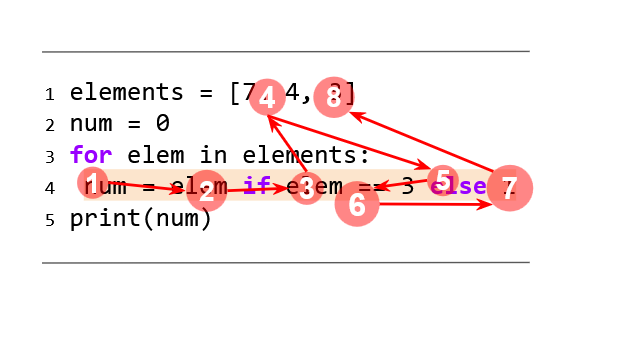
\includegraphics[scale=0.8]{figures/a.png}
  \caption{Obfuscated code snippet \citet{silva2023evaluating}}
  \label{fig:AnhangsChor}
\end{figure}

\begin{figure} [H]
  \centering
  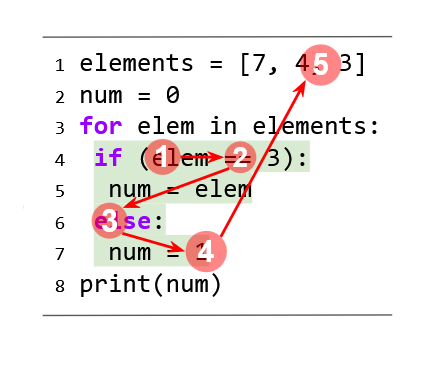
\includegraphics[scale=0.8]{figures/b.png}
  \caption{Clarified version \citet{silva2023evaluating}}
  \label{fig:AnhangsChor}
\end{figure}


\subsubsection{Program Comprehension: Iteration vs. Recursion} 
The study \citet{aroobaunderstanding} investigates how students perceive recursive and iterative programs and analyzes their cognitive processes and visual attention \citet{aroobaunderstanding}. Moreover, the study inspected whether students followed a top-down approach or bottom-up approach.
The results present that there was no significant difference between recursive and iterative programs in terms of code comprehension \citet{aroobaunderstanding}.  However, visual attention differed between iteration and recursion. 

\subsubsection{Cognitive Load and Code Complexity} 

The eye-tracking paper \citet{abbad2022estimating} investigates how to identify difficult areas of code for programmers.  Participants were given different Java code snippets and mentioned the areas of the code they found difficult \citet{abbad2022estimating}. Researchers compared the eye-tracking data with the parts marked as complicated by the participants. With the collected data, they trained machine learning models to forecast which parts of the code would challenge code comprehension \citet{abbad2022estimating}. The researches achieved more than 86\% accuracy in predicting complicated parts of code snippets. The study highlights its future usage for developing tools that can enhance code review and adaptive e-learning. 



\subsubsection{Code Structure and Indentation} 


The eye-tracking study \citet{bauer2017indentations} investigates how indentation affects comprehension. Participants analyzed Java code snippets with different levels of indentations: 0, 2, 4, and 8-space. The results presented no significant relationship between comprehension and indentation \citet{bauer2017indentations}. However, the most correct answers were given when the participants analyzed code with 4-space indentation . Furthermore, the results indicated that 8-space indentation was rated as the easiest to read level of indentation, but did not improve the accuracy of the correct answers \citet{bauer2017indentations}. Overall, eye-tracking data showed no significant differences in gaze patterns across different indentation levels, and the study highlights the need for further investigation. 



Another study \citet{yorimoto2024quantitative} investigates how indentation affects code comprehension. Students were given code tasks with different levels of indentation: 0-character, 4-character, and random indentation \citet{yorimoto2024quantitative}. The researchers measured the eye movements and cognitive load of the participants. The results showed increased confusion and cognitive load when students analyzed code with unstructured indentation \citet{yorimoto2024quantitative}. Furthermore, 4-character indentation resulted in more precise but longer focus on code areas. The study mentions that indentation had little impact on small code tasks and highlights that further investigation is needed \citet{yorimoto2024quantitative}.   
\subsubsection{Code comments} 

This study \citet{bakhuizen2019comments}. investigates how incorrect code comments affect programmers' code comprehension. Participants analyzed code containing missing, incorrect, or correct comments.
The researchers used eye-tracking technology to measure how often participants read code comments. The results indicate that participants read code comments as frequently as the code \citet{bakhuizen2019comments}. Furthermore, incorrect comments can negatively affect code comprehension, leading to misinterpretations of the code. Moreover, accurate and correct comments are useful when they provide correct information for unknown functions. 

The reviewed key studies present that eye-tracking technologies effectively investigate code comprehension.  Eye-tracking data provide insights into how expert and novice programmers perceive different code structures and styles. There has been made significant progress in investigating the comprehension and readability of code by programmers.  However, there is a lack of deeper researcher on how indentation and comments influence the comprehension. 
This thesis analyzes how indentation and comments impact computer science students’ perception of code comprehension.  


\chapter{Study Design}



\section{Methodology}

\subsection{Study Approach}

The data in this study is gathered using two methods: eye-tracking technology and questionnaire. This approach provides both objective and subjective data, as well as quantitative and qualitative data.
Eye-tracking technology gives objective data. Using this type of data, it can be tracked which parts of the code are seen and for how long. Furthermore, cognitive load can be measured.
On the other hand, questionnaire can give quantitative data (using Likert scale questions). Moreover, questionnaire can give subjective data about the participants (using open-ended questions). The participants report their perceived code comprehension.  
Previous research has also used both methods to gather data for a deeper code comprehension. (see Chapter Literature review). The Figure ... presents an overview how the data is gathered. 



\begin{figure} [H]
  \centering
  
  \caption{Study data}
  \label{fig:AnhangsChor}



\begin{tikzpicture}[node distance=1cm and 3cm, align=center, font=\footnotesize]

% Define the styles for the boxes
\tikzstyle{box} = [draw, minimum height=3cm, minimum width=4cm, text width=3.5cm, inner sep=5pt]

% Create the nodes for Eye-Tracking and Questionnaire
\node (eyeTracking) [box] {Eye-Tracking  data \\[5mm] $\rightarrow$ Measures gaze \\ $\rightarrow$ Measure cognitive load};
\node (questionnaire) [box, right=of eyeTracking] {Questionnaire data \\[5mm] $\rightarrow$ Subjective data  };

% Create the middle box for "The Study"
\node (study) [box, below=2cm of $(eyeTracking)!0.5!(questionnaire)$, text width=7cm, align=center] {The study \\[5mm] $\rightarrow$ Both data give a complete view}; 

% Draw lines from Eye-Tracking and Questionnaire to "The Study"
\draw[->] (eyeTracking) -- (study);
\draw[->] (questionnaire) -- (study);

\end{tikzpicture}

\end{figure}

 




The study consists of two formats: an eye-tracking study (offline study) and an online study without eye-tracking. The Figure ... presents the structure of the study.

\begin{figure} [H]
  \centering
  
  \caption{Study structure}
  \label{fig:AnhangsChor}


\begin{tikzpicture}[node distance=1.5cm, font=\footnotesize, align=center]

% Create the side-by-side rectangles for Eye-Tracking, Questionnaire, and Questionnaire2
\node (eyeTracking) [draw, minimum height=2cm, minimum width=3cm, text width=2.5cm, align=center] {Eye-Tracking};
\node (questionnaire) [draw, minimum height=2cm, minimum width=3cm, text width=2.5cm, align=center, right=1.5cm of eyeTracking] {Questionnaire};
\node (questionnaire2) [draw, minimum height=2cm, minimum width=3cm, text width=2.5cm, align=center, right=1.5cm of questionnaire] {Questionnaire};

% Create the Offline Study rectangle, below Eye-Tracking and Questionnaire
\node (offlineStudy) [draw, minimum height=2cm, minimum width=3cm, text width=3cm, align=center, below=1.5cm of eyeTracking] {Offline study};

% Create the Online Study rectangle, below Questionnaire2
\node (onlineStudy) [draw, minimum height=2cm, minimum width=3cm, text width=3cm, align=center, below=1.5cm of questionnaire2] {Online study};

% Create the center Study rectangle
\node (study) [draw, minimum height=2cm, minimum width=6cm, text width=6cm, align=center, below=1.5cm of $(onlineStudy)!0.5!(offlineStudy)$] {The study };

% Draw arrows from Eye-Tracking, Questionnaire, and Questionnaire2 to their respective study
\draw[->] (eyeTracking) -- (offlineStudy);
\draw[->] (questionnaire) -- (offlineStudy);
\draw[->] (questionnaire2) -- (onlineStudy);

% Draw arrows from Online Study and Offline Study to the center Study
\draw[->] (onlineStudy) -- (study);
\draw[->] (offlineStudy) -- (study);

\end{tikzpicture}
\end{figure}

The eye-tracking study (offline study) gathers data using eye-tracking technology and a questionnaire. The eye-tracking device gives objective quantitative data as output and the questionnaire gives both objective and subjective data, as well as quantitative and qualitative data as output.  By combining both methods, the findings indicate whether questionnaire data aligns with the eye-tracking data.
The online study without eye-tracking gathers data using only questionnaire. By using both formats, the study gives a more comprehensive overview of how computer science students perceive code. 



\subsection{Code Snippet Selection}

The programming language used for the code snippets is Java, since it is a widely used language.  Additionally, most students, which participated in the study, are from LMU University, where Java is a key part of many computer science courses. The following code snippets formats are used in the study:



\begin{enumerate}
    \item \textbf{Comment formats:}
    \begin{itemize}
        \item \textbf{No comments:} Code snippet without any comments.
        \item \textbf{Minimal comments:} Code snippet with minimal and essential comments.
        \item \textbf{Helpful comments:} Code snippet with meaningful comments.
        \item \textbf{Redundant comments:} Code snippet with unnecessary comments.
    \end{itemize}
    
    \item \textbf{Levels of indentations:}
    \begin{itemize}
        \item \textbf{0-spaces indentation (no indentation):} Code snippet without indentation.
        \item \textbf{4 spaces indentation:} Code snippet with 4-spaces indentation.
        \item \textbf{Random indentation:} Code snippet with inconsistent indentation.
    \end{itemize}
\end{enumerate}

Figure .............  presents an example for one code snippet with minimal comments . All code snippets used in the study are provided in Appendix A.


\begin{figure} [H]
  \centering
  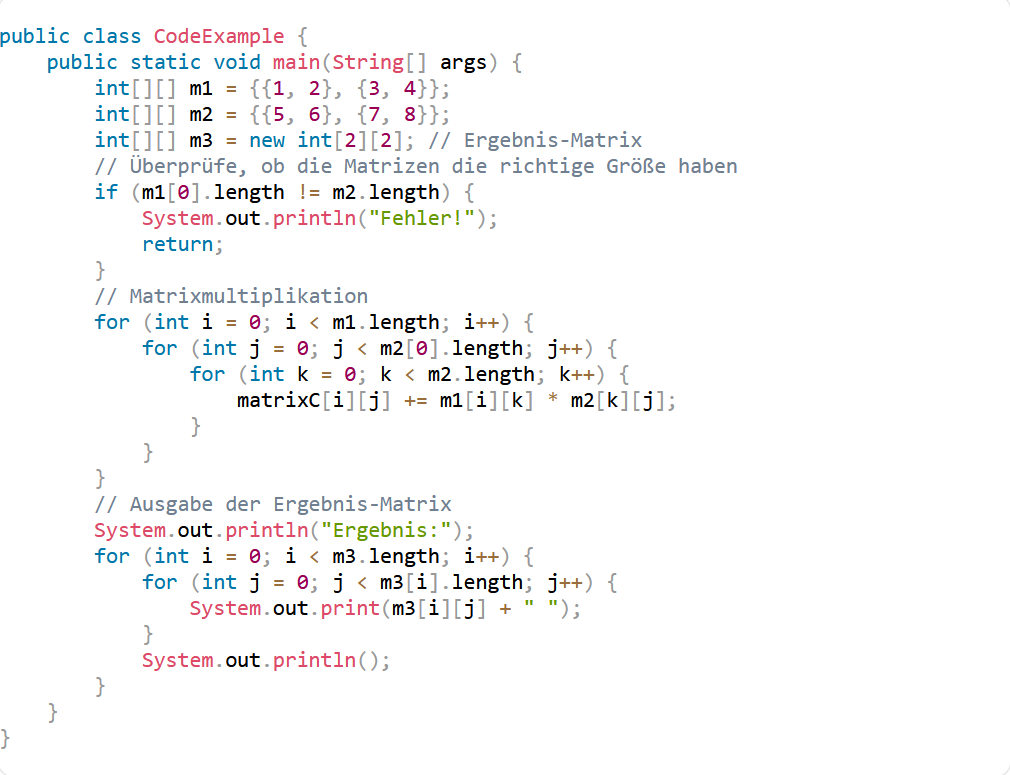
\includegraphics[scale=1.1]{figures/codeb.png}
  \caption{Code snippet example }
  \label{fig:AnhangsChor}
\end{figure}

\subsection{Justification of code snippets selection }
The code snippets are collected from programming lectures conducted at LMU University and adapted from the computer science exercises. The main reason why the snippets were selected from lectures is that they provide widely used examples. These examples are suitable for investigating code comprehension.  
The selection of the code snippets formats is based on the findings from previous research. It is defined that indentation levels and comment styles influence code readability and comprehension.  (e.g., Chapter Literature review). Therefore, the snippets in this study are designed to investigate how different levels of indentations and different commenting formats affect code comprehension.  Moreover, the code snippets are simple enough, and no additional knowledge is required. Furthermore, the usage of loops and conditionals in the snippets requires different levels of cognitive processing.    


Each snippet is focused on one dimension at a time (levels of indentations or commenting formats). This enables a simple analysis and comparison across the different formats. The study has seven different code snippets. It combines three levels of indentation and four types of commenting styles. For the commenting formats, four types are selected.  The role of the snippet with no comments is to investigate whether code can be understood without any additional information.  Minimal comments test whether minimal information is better than none and improves comprehension, or makes it difficult for understanding.
Helpful comments investigate whether meaningful information enhances deeper code comprehension. Redundant comments tend to explore whether unnecessary comments make the code difficult to understand, causing cognitive overload.


For the indentation, three levels were selected. 
The role of the code snippet with no indentation is to investigate how the absence of indentation influences code readability and whether it causes cognitive overload.
The 4-space indentation is defined as standard indentation in research and tends to explore whether it enhances deeper code readability.  
Random indentation tests whether using different indentation across the code makes the snippet difficult to read and causes cognitive overload.


For the commenting formats snippets, the snippets have 4-space indentations. This ensures that the focus is only on the comments. This indentation is defined as a "control group", which allows deeper comparison across the different commenting formats. 
For the indentation code snippets, the snippets consist of no comments. This ensures that the focus is only on the indentation. Here the no comment format is also defined as a "control group", which allows deeper comparison across the different indentation levels. An overview is presented in Table ....


\begin{table}[ht]
\centering
\caption{Overview of code snippet formats}
\begin{tabular}{|p{6cm}|p{6cm}|}

\hline
\multicolumn{2}{|c|}{
\textbf{Commenting formats}} \\
\hline
Type & Control Variable \\
\hline 
No comments & 4-space indentation \\
Minimal comments & 4-space indentation \\
Helpful comments & 4-space indentation \\
Redundant comments & 4-space indentation \\
\hline
\multicolumn{2}{|c|}{\textbf{Indentation levels}} \\
\hline
Type & Control Variable \\
\hline
No indentation & No comments \\
4-space indentation & No comments \\
Random indentation & No comments \\
\hline
\end{tabular}
\label{tab:snippet_control}
\end{table}



\subsection{Technical setup}

The eye-tracking study (offline study) was conducted at LMU, Munich. As eye-tracking device was used a Pupil Labs Core. This device contains glasses with three cameras. The glasses were connected to a laptop, running Pupil Capture software. This software ensures calibration and recording of eye movements. The laptop was placed on a desk. During the study, participants read the snippets and answered the questionnaire on the same laptop. This setup ensured minimal distractions.  The technical setup is presented in Figure ….

\begin{figure} [H]
  \centering
  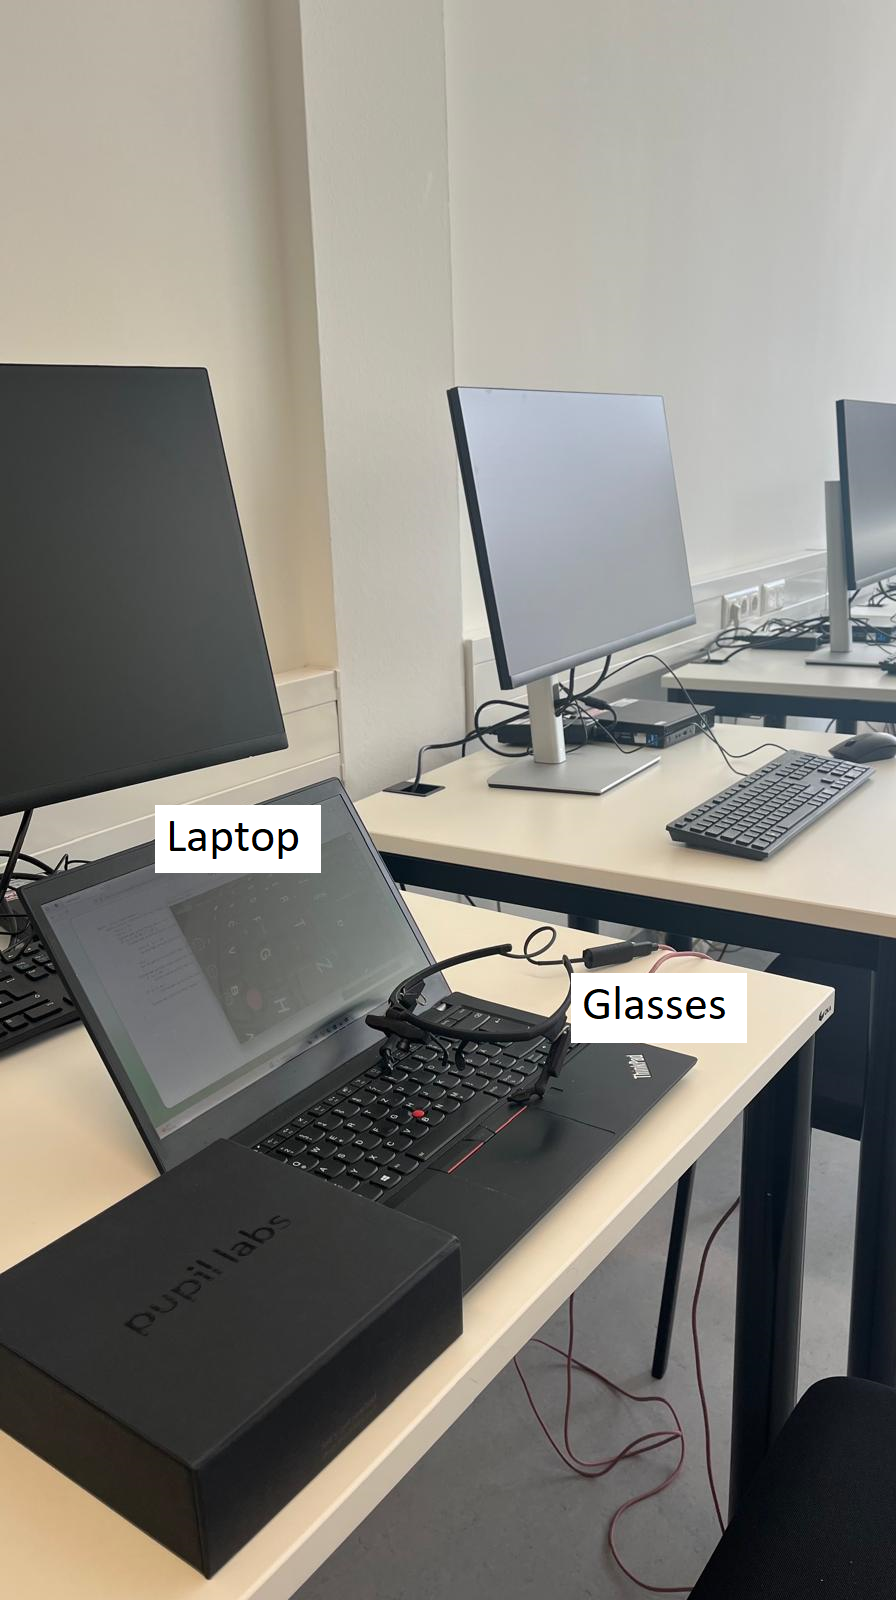
\includegraphics[scale=0.6]{figures/setup.png}
  \caption{Technical setup }
  \label{fig:AnhangsChor}
\end{figure}



\subsection{Research Variables}



\section{Questionnaire Design}


\subsection{First part of Questionnaire}
The first part of the questionnaire gives general information about the participants. 
Participants provide details about their field of study, as well as information about their academic background: their programming experience level and experience in Java.

\begin{figure} [H]
  \centering
  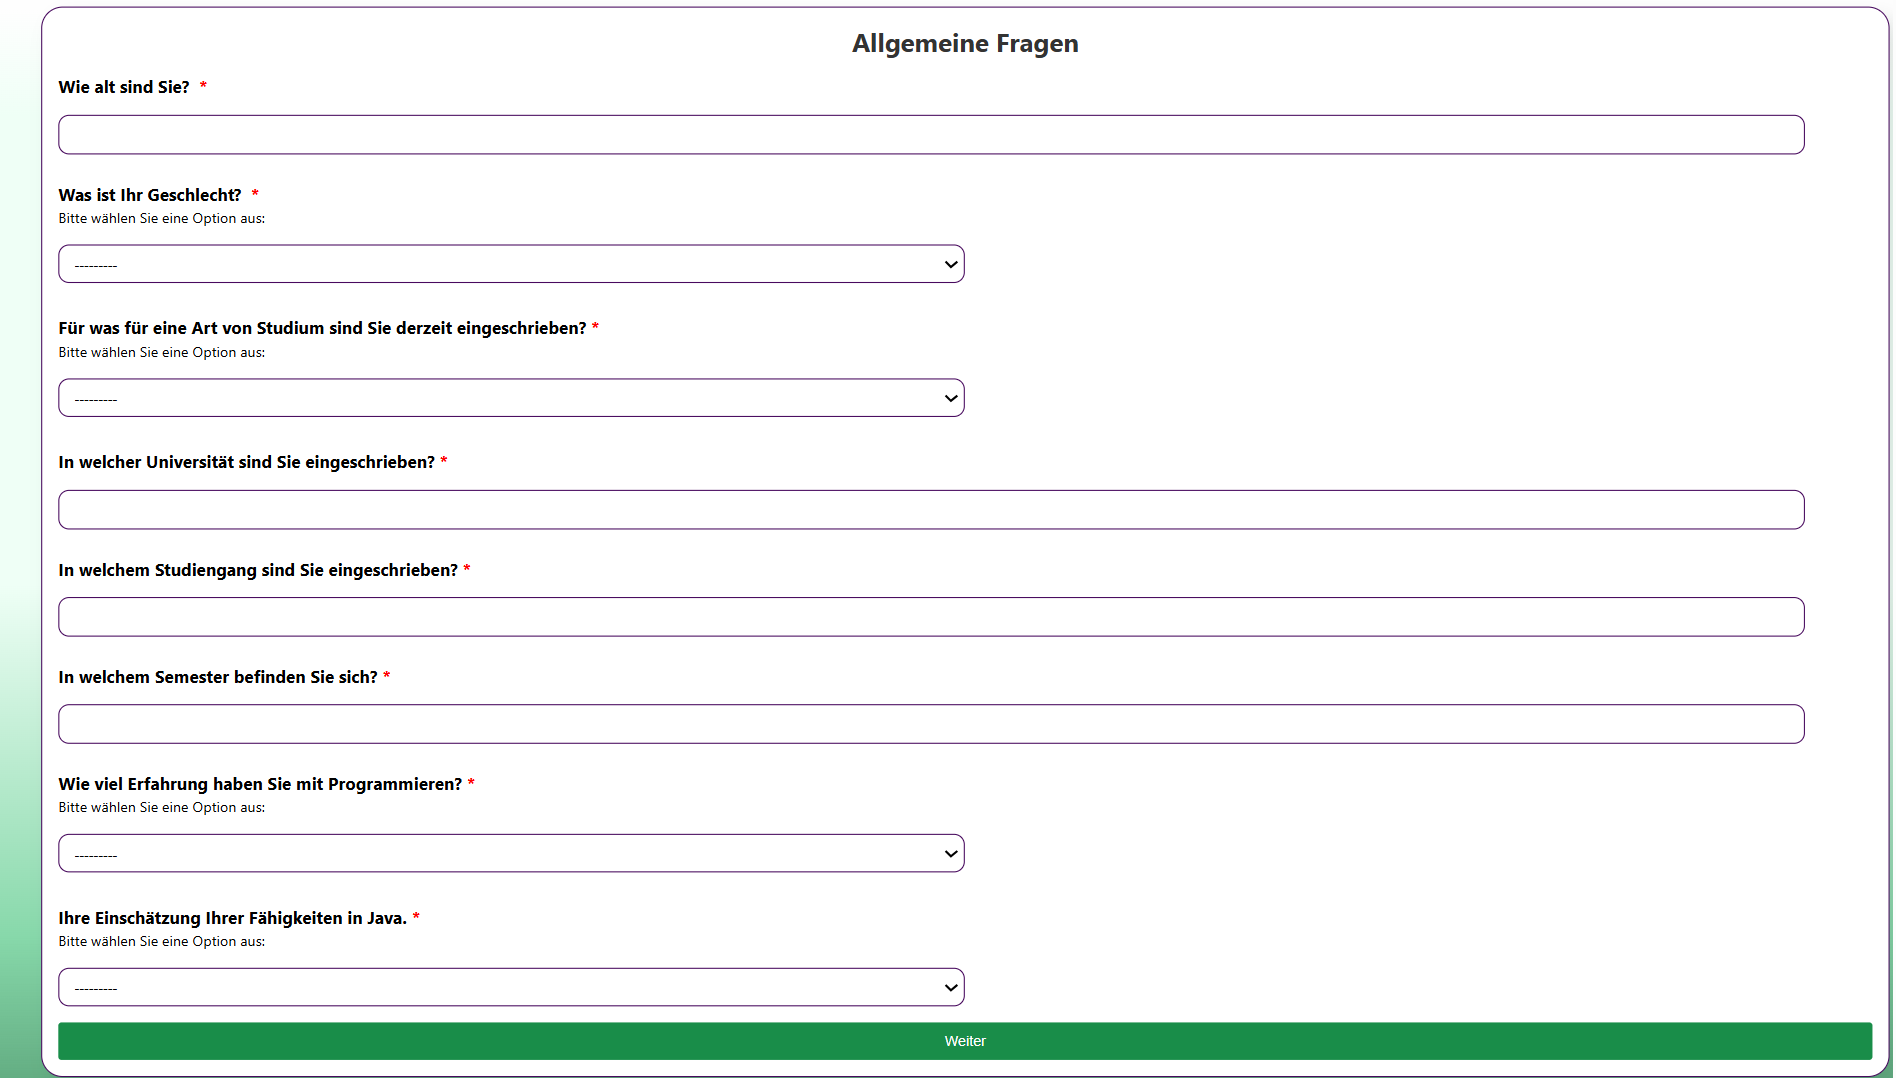
\includegraphics[scale=0.45]{figures/allgemein.png}
  \caption{First part of Questionnaire}
  \label{fig:AnhangsChor}
\end{figure}


\subsection{Main part of Questionnaire}

In the main part of the questionnaire are shown seven different code snippets. Their order is randomized to avoid bias. Each code snippet presents a different level of indentation and a different type of comment format.
Participants answer five questions corresponding to each code snippet. These questions are related to the code snippet’s function, ratings of the code comprehension, code indentation, and code commenting.


\begin{figure} [H]
  \centering
  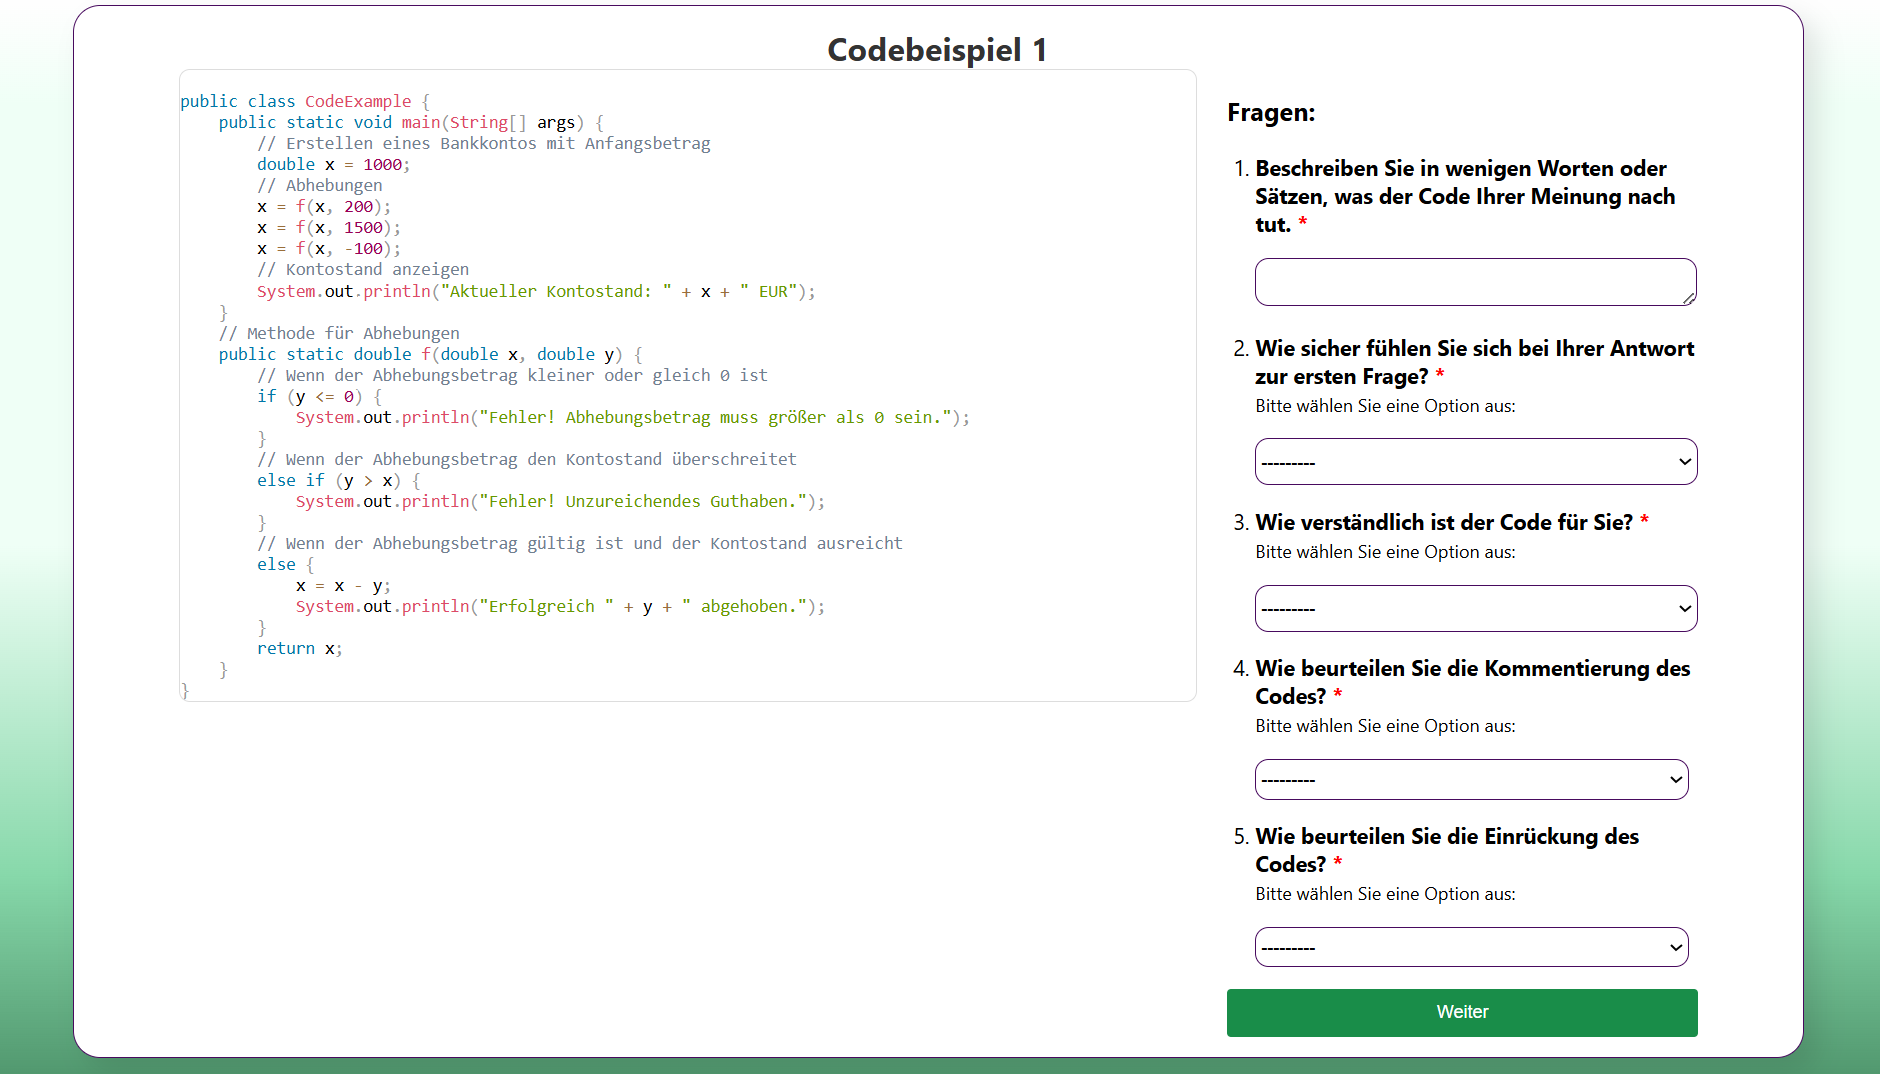
\includegraphics[scale=0.45]{figures/main_p.png}
  \caption{Main part of Questionnaire}
  \label{fig:AnhangsChor}
\end{figure}



\subsection{Final part of the Questionnaire}
In the last part of the questionnaire, participants give their opinions on code indentation and code comments guidelines. They describe what they take into consideration when defining poorly commented and well-commented code. Moreover, they explain which code indentation style they use.  


\begin{figure}  [H]
  \centering
  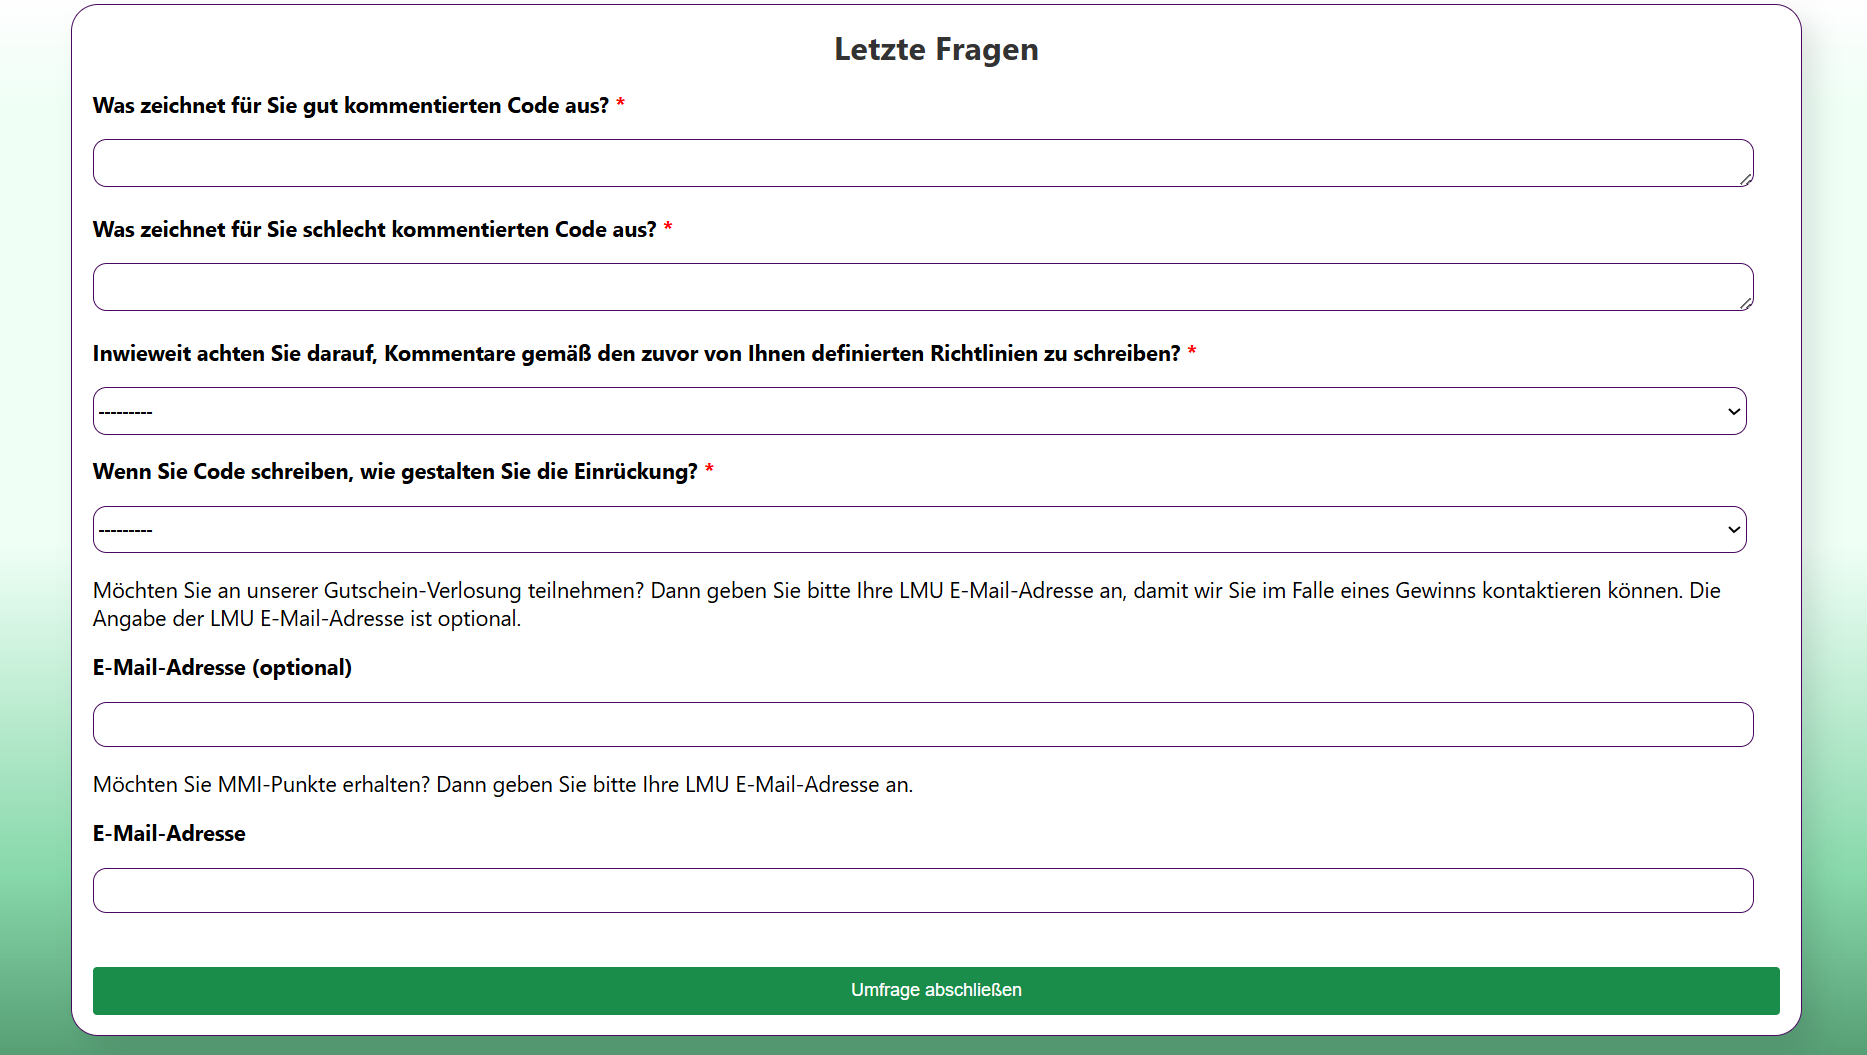
\includegraphics[scale=0.45]{figures/last_part.png}
  \caption{Final part of the Questionnaire}
  \label{fig:AnhangsChor}
\end{figure}


 
\section{Procedure}

The eye-tracking study (offline study) and the online study without eye-tracking formats are constructed similarly, but have some differences. The detailed procedure for both formats is outlined below.

\subsection{Procedure for the Eye-Tracking Study}




\begin{enumerate}
    \item \textbf{Introduction:} At the beginning, participants answered several warm-up questions: “How are you feeling today? Do you have any experience with reading source code? Do you have any experience with eye-tracking studies?”  Then, participants are informed about the purpose of the study, data collection methods, and their right to withdraw from the study at any time.

    \item \textbf{Calibration of the Eye-Tracking System:} 
    Eye-tracker calibration is essential to ensure that the eye-tracking device correctly detects participants’ eyes and eye movements. Before calibration, participants put on the eye-tracking device and adjust three cameras: one for the screen, one for the right eye, and one for the left eye. It is essential to ensure that both eyes are correctly detected. After the adjustment is performed, participants are asked to focus on several specific points on the screen. The system records their gaze. In some cases, calibration errors occurred and recalibration was required. After the calibration is completed, the eye-tracking system started recording participants’ gaze. Participants read all relevant information themselves and then they proceeded to the questionnaire.
    
    \item \textbf{First part of Questionnaire:}  
    Participants answered several questions providing demographic, background, and programming experience information. When the students filled out these questions, they proceeded to the main part of the Questionnaire - Code Comprehension Task.

    \item \textbf{Main part of Questionnaire - Code Comprehension Task:}  Each participant is shown seven different code snippets. The order of the code snippets was randomized in order to avoid bias. The participants read each code snippet, while the eye-tracking device recorded their gaze movements, saccades, fixations, and pupil dilation. After reading each code snippet, students answered five questions. These questions are related to the corresponding code snippet. Moreover, their answers and response times were recorded.

    \item \textbf{Final part of the Questionnaire:} 
    The participants answered several questions providing information about their opinions on commenting and indentation in code.

    \item \textbf{End of the study:} 
    Participants are asked to give feedback on the difficulty level of the code snippets. Furthermore, the students mentioned their opinions on code readability and code comprehension. Additionally, they shared the challenges they faced during the eye-tracking study.

\end{enumerate}


\subsection{Procedure for the Online Study without Eye-Tracking}


\begin{enumerate}
    \item \textbf{Introduction} Participants are informed about the purpose of the study, data collection methods, and their right to withdraw from the study at any time. Participants read all relevant information themselves and then they proceeded to the questionnaire.
    
    \item \textbf{First part of Questionnaire:}
    Participants answered several questions providing demographic, background, and programming experience information. When the students filled out these questions, they proceeded to the main part of the Questionnaire - Code Comprehension Task.

    \item \textbf{Main part of Questionnaire - Code Comprehension Task:} Each participant is shown seven different code snippets. The order of the code snippets was randomized in order to avoid bias. The participants read each code snippet. After reading each code snippet, students answered five questions. These questions are related to the corresponding code snippet. Since there was no eye-tracking device, only their answers and response times were recorded.

    \item \textbf{Final part of the Questionnaire:}
    The participants answered several questions providing information about their opinions on commenting and indentation in code.
\end{enumerate}






\section{Measurements}

\section{Participants}


\section{Ethical Considerations}

\begin{enumerate}
    \item \textbf{Informed Consent: }All participants receive clear information about the purpose of the study. The participants have the right to withdraw at any time.
    
    \item \textbf{Data Protection}
    \begin{itemize}
        \item Demographic information, such as gender and age, is collected.
        \item If participants choose to receive compensation from the university, they provide their university email address.
        \item The rest of the data is anonymized and is stored for a maximum of three years.
        \item Non-anonymized data is stored for a maximum of three years.
        \item All collected data is encrypted.
        \item For eye-tracking participants, video recordings and gaze data are stored.
        \item For all participants, their questionnaire responses are stored.
        \item At any time, participants can request deletion of their data.
        \item No personal data is shared with third parties.
    \end{itemize}
\end{enumerate}

\chapter{Results}

\chapter{Discussion - Interpretation of Results}

\section{Limitations} 
Both formats of the study have several limitations that may have an impact on the results.
In the eye-tracking study only .... 10..... computer science students participated.  This small number of participants limited the generalization of the findings.  Moreover, some participants moved their heads too much.  These movements caused an inaccuracy in gaze patterns and calibration errors. Furthermore, several technical issues with eye-tracking device were reported. Sometimes the changes of ambient and screen lighting led to inaccuracy of the records.
The online study without eye-tracking also has several limitations that may have an impact on the results. 
Only .....30..... computer science students participated in the study. The small number of participants limited the generalization of the results. 
Moreover, some participants did not answer all questions. Therefore, only part of their answers were recorded, which led to missing data. 
Furthermore, the online study was not conducted in a controlled environment. Participants filled out the questionnaire in different environments, which may have an influence on their answers.  
These limitations highlight that improved technical setup and future research is needed. 


\section{Improvements}

Several improvements can be considered. First, a larger number of participants would provide more clear generalization of the findings. Additionally, the use of chin supports in the eye-tracking study may minimize participants’ head movements. It is also important to ensure consistent lighting conditions while conduction the eye-tracking study. Another suggestion is to select a laptop device that is less sensitive to ambient and screen lighting. This suggestion may reduce records errors. By implementing these improvements, future research can enhance clear generalization of the findings. 

\chapter{Conclusion and Outlook}
\label{sec:conclusion}
